\documentclass[a4paper, 12pt, twoside]{article}
\usepackage[utf8]{inputenc}		
\usepackage[T1]{fontenc}		
\usepackage[francais]{babel}
\usepackage{lmodern}
\usepackage{ae,aecompl}
\usepackage[top=2.5cm, bottom=2cm, 
			left=3cm, right=2.5cm,
			headheight=15pt]{geometry}
\usepackage{graphicx}
\usepackage{eso-pic}	
\usepackage{array} 
\usepackage{hyperref}
\input{pagedegarde}

\title{Dopamine-Guard : Système de régulation assisté par IA}
\entreprise{Projet d'Informatique L1}
\datedebut{Février 2026}
\datefin{Mai 2026}

\membrea{SELAMBAYE Maxime 45001766}
\membreb{NDIAYE Djibril Oumar 45007559}
\membrec{BOUILLY Matheo  45015077}
\membred{LE LANN Orian 45002999}
\membree{Lien GitHub : \url{https://github.com/45001766-prog/Dopamine-Guard}}

\begin{document}
\pagedegarde


\tableofcontents
\newpage

\section{Introduction}
Nous vivons une époque où nos cerveaux sont devenus la ressource la plus convoitée au monde. Ce que nous appelons familièrement "faire une session de jeu" ou "passer du temps sur PC" est en réalité le résultat d'une ingénierie de pointe conçue pour nous maintenir dans un état de transe cognitive. Ce phénomène ne se limite plus aux jeunes générations : si les plus âgés étaient initialement réticents face aux technologies, leur temps passé devant les écrans et les jeux grand public a bondi de 150 \% en deux ans (Source : Pew Research Center). L’addiction numérique est devenue universelle.


Le problème est alarmant pour notre productivité : un étudiant qui interrompt ses révisions pour une "courte session sur PC" met en moyenne 23 minutes et 15 secondes à retrouver sa concentration initiale (Source : University of California, Irvine). Biologiquement, le constat face au moniteur est encore plus frappant : absorbé par l'écran, notre rythme de clignement d'yeux chute de 20 à seulement 5 ou 7 par minute, provoquant une sécheresse oculaire sévère et verrouillant littéralement notre cerveau dans une hypnose numérique (Source : University of Iowa Health Care).

Face à des environnements virtuels si immersifs qu'ils dépassent la volonté humaine, les logiciels de blocage parental ou les minuteurs classiques ont échoué. Ils imposent une censure brutale qui crée de la frustration et pousse systématiquement au contournement. Dans le cadre de notre projet de groupe, nous avons conçu Dopamine-Guard, une approche radicalement innovante et subtile. Notre idée n’est pas de déconnecter l’utilisateur de force ou de couper son ordinateur en plein milieu d'une action.

En couplant la vision par IA à la rapidité du langage C sous Linux, notre système d'alerte détecte directement les signaux physiques de la transe (chute du rythme palpébral, fixité du regard, affaissement du cou vers le moniteur). Plutôt que d'interdire, notre programme en C va dégrader chirurgicalement le plaisir de l'expérience en agissant directement sur le système graphique : les couleurs de l'écran se ternissent progressivement, la fluidité d'affichage s'effondre, un léger lag de traitement apparaît. Dopamine-Guard renders l'immersion techniquement médiocre. L'utilisateur ne se sent pas censuré, il ressent simplement de la fatigue visuelle et de l'ennui technique. Il décide alors, de lui-même, de fermer ses applications pour reprendre le contrôle de son temps et de sa productivité.

\newpage

\section{Description du projet et objectifs}

\subsection{Présentation Générale de l'Application}
Le projet Dopamine-Guard consiste à développer un logiciel de bureau pour ordinateur capable de moduler l'affichage de l'écran en fonction du comportement de l'utilisateur. Techniquement, l'application se divise en deux grands modules qui fonctionnent en continu : un module d'analyse visuelle par Intelligence Artificielle et un module d'action codé en langage C. Le programme utilise la webcam pour capter les expressions du visage, puis traite ces informations pour vérifier si l'utilisateur est fatigué ou s'il est bloqué depuis trop longtemps devant une activité très immersive (comme un jeu vidéo). Si le logiciel valide cet état de fixation, il communique directement avec la carte graphique et le système d'affichage de l'ordinateur. L'application applique alors des modifications visuelles, comme le passage de l'écran en noir et blanc ou l'apparition de légers ralentissements (lags). L'idée n'est pas de couper l'ordinateur de force, mais de rendre l'écran moins stimulant pour inciter l'utilisateur à faire une pause de lui-même.

\subsection{Les Objectifs Fonctionnels et Comportementaux}
Cette partie définit ce que l'application doit réaliser concrètement pour aider l'utilisateur au quotidien :
\begin{itemize}
    \item \textbf{Mesure biométrique simple :} Le premier but est d'utiliser une simple webcam de bureau pour analyser l'utilisateur. Le programme doit être capable de compter le nombre de clignements d'yeux par minute et de détecter si la tête penche trop en avant, sans que l'utilisateur n'ait besoin de porter un équipement spécial.
    \item \textbf{Réaction progressive de l'écran :} L'application ne doit pas punir l'utilisateur d'un coup. Nous voulons mettre en place des paliers. Si l'utilisateur commence à s'endormir ou à trop fixer l'écran, les couleurs s'en vont doucement. S'il reste bloqué, les micro-ralentissements s'activent pour casser la fluidité de son jeu ou de sa navigation.
    \item \textbf{Respect du travail de l'utilisateur :} Le système doit être assez intelligent pour faire la différence entre un étudiant très concentré qui tape un code ou lit un cours, et un utilisateur passif bloqué devant une boucle de vidéos ou un jeu. L'action du logiciel ne doit se déclencher que dans le second cas.
\end{itemize}

\subsection{Les Objectifs Techniques (Cahier des Charges)}
Cette sous-partie regroupe les défis informatiques que notre groupe doit résoudre pour que le logiciel fonctionne correctement :
\begin{itemize}
    \item \textbf{Contrôle de l'affichage en langage C :} Notre objectif principal est d'utiliser la rapidité du langage C pour modifier l'écran sous Linux (Ubuntu). Nous devons apprendre à utiliser des bibliothèques système comme Lib-X11 pour changer les couleurs ou la fluidité de l'affichage directement, sans avoir besoin de créer une interface graphique lourde.
    \item \textbf{Utilisation du Multi-Threading :} Pour éviter que notre analyse d'image par l'IA ne fasse ramer l'ordinateur (surtout si l'utilisateur joue à un jeu vidéo en même temps), nous devons séparer le code en deux fils d'exécution indépendants (threads). L'IA tournera d'un côté, et le contrôle de l'écran en C de l'autre.
    \item \textbf{Stabilité et gestion de la mémoire :} Comme notre programme a pour but de tourner en tâche de fond pendant plusieurs heures, nous devons faire très attention à la gestion de la mémoire vive (RAM). Nous utiliserons l'outil Valgrind pour vérifier qu'il n'y a aucune fuite de mémoire dans notre code C, ce qui pourrait faire crasher le PC.
\end{itemize}

\newpage

\section{Environnement de travail}

\begin{figure}[h]
\centering
\includegraphics[width=0.8\textwidth]{schema_architecture.png} 
\caption{Architecture du flux d'information de Dopamine-Guard.}
\label{schema}
\end{figure}

\subsection{Architecture Technique et Système de Régulation Comportementale}
Pour ce logiciel de bureau, le choix du langage C/C++ est fondamental. Il permet d'accéder directement au processeur (CPU) et à la carte graphique (GPU) afin de garantir une analyse d'image fluide en temps réel, tout en nous donnant le pouvoir d'altérer l'affichage de l'ordinateur pour appliquer nos contre-mesures.

\subsection{Langage et Intégration Système Desktop}
Le cœur de notre moteur d'intelligence artificielle et de contrôle matériel est développé en C et C++. Conçu pour la plateforme PC sous Linux (Ubuntu 24.04 LTS), le programme utilise les API natives POSIX pour faire le pont direct entre les flux de la webcam, les calculs de la transe et la gestion de l'affichage vidéo de la machine.

\subsection{Développement de l'Application de Régulation}
L'application fait le lien entre la perception de la webcam et les réactions physiques de l'écran. Elle s'exécute de manière asynchrone pour ne jamais ralentir les autres logiciels ou jeux en cours d'exécution.

\subsection{Gestion du Flux et Multi-Threading}
We use the POSIX Threads library (pthread.h) to split the application execution into two autonomous threads:
\begin{itemize}
    \item \textbf{Le Thread d'Analyse (IA) :} Dédié à la capture vidéo et aux calculs de détection de MediaPipe.
    \item \textbf{Le Thread d'Action (Langage C) :} Tourne en arrière-plan, écoute les scores du premier thread et pilote l'affichage.
\end{itemize}
Cette séparation empêche le système de geler pendant les calculs d'image.

\subsection{Logique de Fonctionnement et Stratégie de Nudging}
L'application fonctionne selon un cycle de régulation continue à deux modes principaux :
\begin{itemize}
    \item \textbf{Mode Surveillance Passive :} Tant que l'utilisateur cligne des yeux normalement et maintient une bonne posture, le programme reste neutre et laisse le système fonctionner au maximum de ses performances.
    \item \textbf{Mode Dissuasion Active (Le Sabotage Invisible) :} Dès que l'Indice de Transe dépasse le seuil critique, le code C applique la stratégie du Nudge. Via les protocoles graphiques Linux, il dégrade subtilement l'expérience (écran terne, micro-lags). Sans subir de censure brutale, l'utilisateur s'ennuie face à un écran devenu inconfortable et décide de lui-même de s'arrêter.
\end{itemize}

\newpage

\section{Bibliothèques, Outils et technologies}
Pour réaliser ce projet, nous avons choisi d'utiliser l'environnement Linux. Ce choix nous permet d'avoir un accès direct aux composants de l'ordinateur, ce qui est nécessaire pour analyser le flux vidéo de la webcam et modifier l'affichage de l'écran en temps réel.

\subsection{Le Langage de Programmation et la Compilation}
\begin{itemize}
    \item \textbf{Le Langage C (Standard C11) :} C'est le cœur de notre application. Nous avons choisi le langage C pour sa rapidité et sa capacité à communiquer facilement avec le système d'exploitation. Il reçoit les données de l'IA, calcule l'indice de transe de l'utilisateur et déclenche les modifications de l'écran.
    \item \textbf{Le Compilateur GCC :} C'est l'outil standard sous Linux qui transforme notre code texte en un programme exécutable par l'ordinateur. Nous l'utilisons avec des options de sécurité (comme -Wall pour afficher tous les avertissements) et d'optimisation (comme -O2) pour que le programme soit le plus efficient possible.
\end{itemize}

\subsection{L'Intelligence Artificielle et le Traitement d'Image}
\begin{figure}[h]
\centering
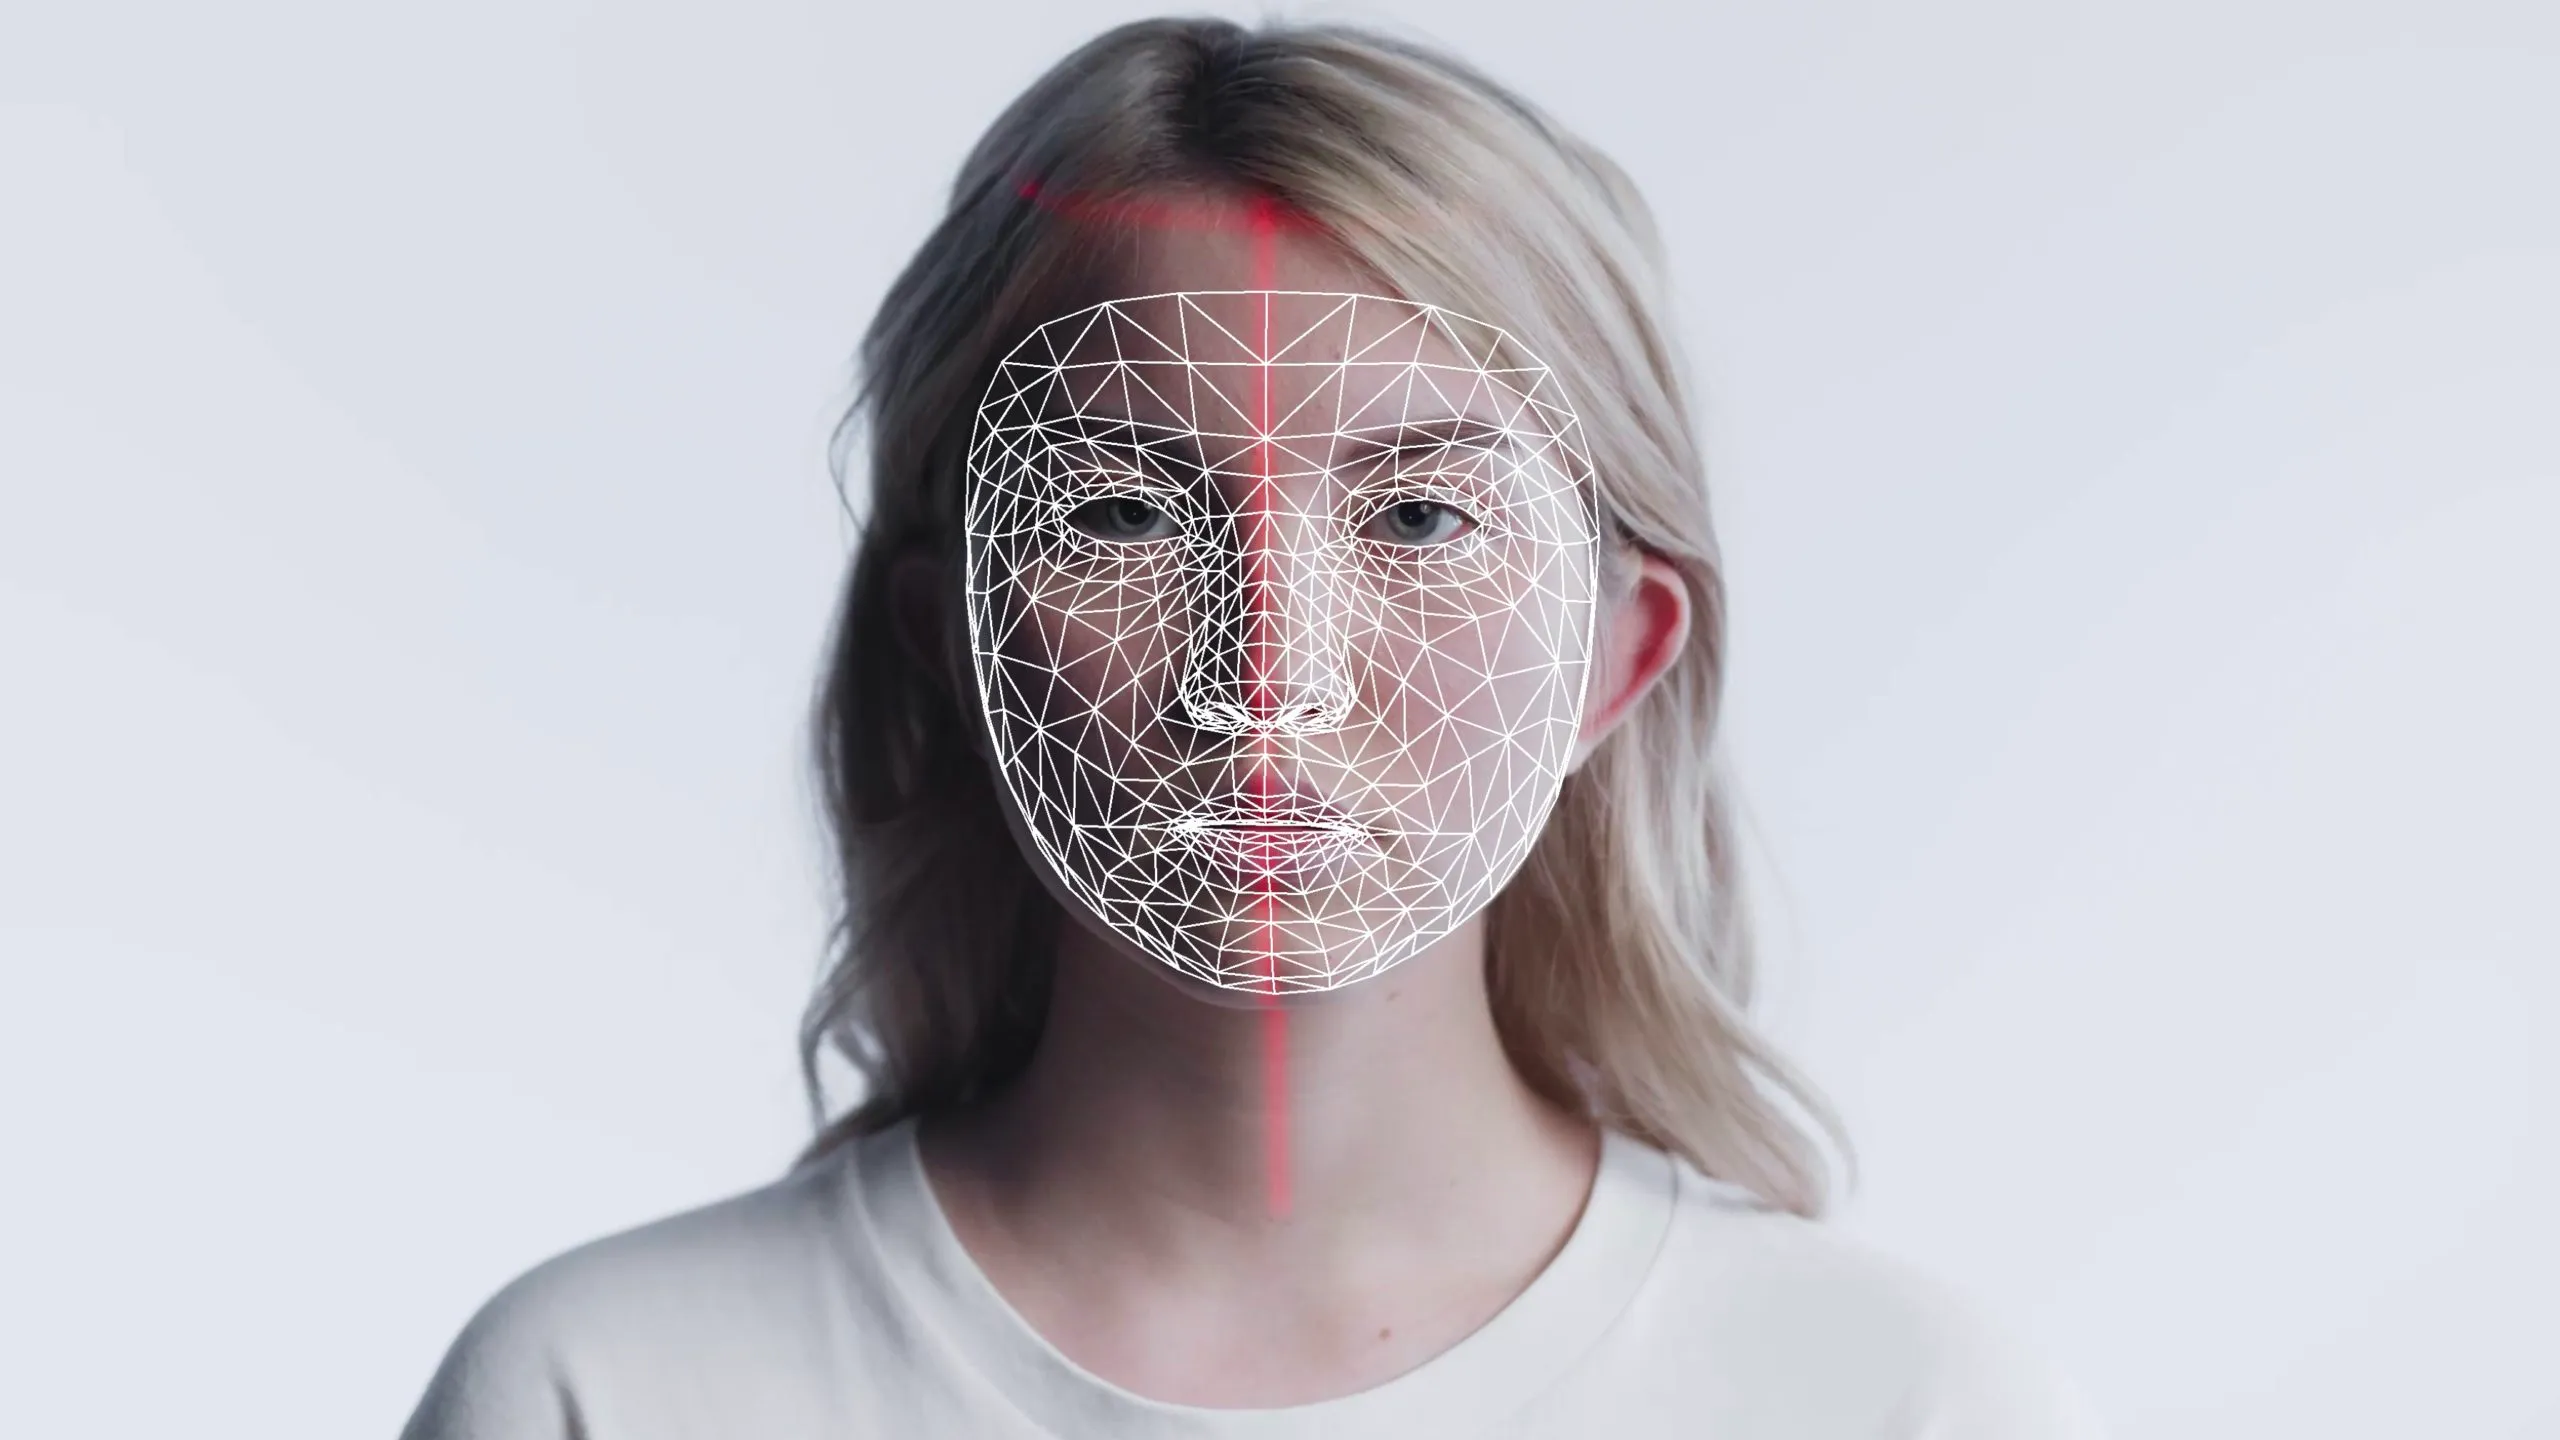
\includegraphics[width=0.4\textwidth]{facemesh.jpg} % Image montrant les 468 points de MediaPipe sur un visage
\caption{Visualisation du maillage facial 3D par MediaPipe.}
\label{facemesh}
\end{figure}

\begin{itemize}
    \item \textbf{MediaPipe Face Mesh (Google) :} C'est l'outil d'Intelligence Artificielle de notre projet. Ce modèle pré-entraîné est capable de trouver et de suivre 468 points précis sur un visage en temps réel. Nous l'utilisons pour mesurer l'écartement des paupières (pour compter les clignements d'yeux) et pour calculer l'angle de la tête afin de détecter une mauvaise posture. Il a l'avantage d'être très léger et de ne pas faire surchauffer le processeur.
    \item \textbf{OpenCV (C++) :} Bibliothèque de référence pour le traitement d'images. Dans notre projet, elle sert d'intermédiaire : elle se connecte à la webcam, récupère le flux vidéo image par image, et redimensionne ces images pour les donner dans le bon format au module MediaPipe.
\end{itemize}

\subsection{Le Contrôle Système et l'Affichage Graphique}
\begin{itemize}
    \item \textbf{Lib-X11 et Xrandr :} Bibliothèques système Linux de bas niveau qui permettent de parler directement au serveur graphique (le système qui gère l'affichage des fenêtres et des écrans). C'est grâce à elles que notre code en C peut modifier la table des couleurs (correction gamma), basculer en mode noir et blanc ou appeler l'altération matérielle sans privilèges root.
    \item \textbf{POSIX Threads (pthread.h) :} Cette bibliothèque permet de faire du "multi-threading", c'est-à-dire de séparer notre programme en deux tâches autonomes qui s'exécutent en même temps. Un premier fil d'exécution gère la webcam et l'IA, tandis qu'un deuxième fil gère le code en C et les modifications de l'écran. Cela évite que l'ordinateur ne se fige pendant les calculs.
\end{itemize}

\subsection{La Communication et les Outils de Diagnostic}
\begin{itemize}
    \item \textbf{Sockets Unix (AF\_UNIX) :} C'est un mécanisme qui permet à deux programmes différents situés sur le même ordinateur de s'envoyer des messages très rapidement. Nous l'utilisons pour créer un "pont" entre le module d'IA (qui détecte les mouvements du visage) et le programme en C (les lignes de code qui décident d'agir sur l'écran).
    \item \textbf{Valgrind :} C'est un outil de diagnostic indispensable en langage C. Comme notre application doit tourner en arrière-plan pendant plusieurs heures, nous utilisons Valgrind pour vérifier que notre programme libère correctement la mémoire vive (RAM) qu'il utilise. Cela nous garantit qu'il n'y a pas de fuites de mémoire qui pourraient ralentir ou faire crasher le PC de l'utilisateur.
    \item \textbf{Système d'Exploitation (Ubuntu 24.04 LTS) :} Cette distribution Linux open-source constitue notre environnement de développement. Elle nous offre tous les outils de programmation nécessaires et nous donne la liberté d'accéder aux couches basses du système pour modifier l'affichage de l'écran sans blocage de sécurité intempestif.
    \item \textbf{L'IA Générative comme Assistant de Code (Gemini Pro) :} Dans le cadre du développement technique, nous avons utilisé l'IA Gemini Pro de Google. Cet outil nous a servi uniquement d'assistant de programmation (pair programming). Il nous a aidés à comprendre les messages d'erreur complexes du compilateur, à structurer correctement la syntaxe des Sockets Unix et à vérifier qu'il ne restait pas de fautes de logique dans l'écriture de nos threads en C.
\end{itemize}

\newpage

\section{Travail réalisé et répartition}
\subsection{Liste des Fonctionnalités Prévues et Réalisées}
\subsubsection*{Fonctionnalités Réalisées}
\begin{itemize}
    \item \textbf{Capture vidéo et prétraitement :} Le programme réussit à se connecter à la webcam, à récupérer le flux en temps réel à 30 images par seconde et à adaptation le format des images pour le module d'analyse.
    \item \textbf{Maillage facial :} L'intelligence artificielle suit correctement les points clés du visage pour extraire les données géométriques de l'utilisateur (ouverture des paupières et inclinaison de la tête).
    \item \textbf{Communication locale :} Le système de Sockets Unix transmet instantanément les données calculées par l'IA vers le programme principal en C sans créer de ralentissement.
    \item \textbf{Gestion du Multi-Threading :} L'intégration de la bibliothèque pthread.h permet de séparer les tâches. L'analyse de la webcam et le contrôle de l'écran tournent en même temps de manière fluide.
    \item \textbf{Contre-mesure de Prévention :} Le code en C modifie les couleurs de l'écran pour passer l'affichage en noir et blanc lorsque le premier seuil de fatigue ou de transe est franchi.
    \item \textbf{Injection de micro-lags graphiques :} Intégration logicielle de temporisations progressives appliquées directement dans la boucle d'action système en C pour casser le confort visuel de manière ciblée en cas de transe critique.
\end{itemize}

\subsubsection*{Fonctionnalités Non Réalisées / Écartées}
\begin{itemize}
    \item \textbf{Filtre de flou visuel dynamique :} Appliquer un flou en temps réel sur tout l'écran demande d'écrire des scripts graphiques très avancés (Shaders OpenGL). Le délai d'implémentation était trop court pour notre niveau actuel.
\end{itemize}

\subsection{Répartition Réelle du Travail}
Pour ce projet de groupe, nous avons séparé le travail en quatre pôles distincts selon les compétences et les intérêts de chacun :
\begin{itemize}
    \item \textbf{Maxime :} S'est occupé de toute la partie vision par ordinateur. Il a configuré OpenCV pour la gestion de la caméra et a mis en place le modèle MediaPipe pour le suivi des points clés du visage.
    \item \textbf{Djibrill :} S'est chargé du traitement mathématique des données de l'IA. Il a écrit les algorithmes et les formules nécessaires pour calculer précisément le taux de clignement d'yeux et l'angle d'inclinaison de la tête.
    \item \textbf{Mathéo :} A développé le programme principal en C. Il a programmé la connexion avec le système graphique Linux (Lib-X11/Xrandr) pour réussir à basculer l'écran en noir et blanc, incluant l'implémentation des micro-lags, et a géré la logique algorithmique des seuils de transe.
    \item \textbf{Orian :} A géré la liaison et l'optimisation générale du projet. Il a créé les Sockets Unix pour faire communiquer le script d'IA avec le code en C, a implémenté le Multi-Threading pour l'exécution simultanée des tâches, et a utilisé Valgrind pour vérifier la mémoire.
\end{itemize}

\newpage

\section{Difficultés rencontrées}
Au cours du développement de ce projet, notre groupe a été confronté à plusieurs obstacles techniques, principalement liés à la communication entre nos scripts et à la gestion de l'affichage sous Linux.

\subsection{La communication entre l'IA et le code C}
La première difficulté majeure a été de faire communiquer notre module d'Intelligence Artificielle (qui traite les images de la webcam) avec notre programme principal en C (qui gère les actions sur l'écran). Au départ, nous pensions faire écrire l'IA dans un fichier texte que le code C lire en boucle. Cependant, cette méthode était beaucoup trop lente et bloquait la fluidité du système. Nous avons dû faire des recherches pour comprendre et mettre en place les Sockets Unix. Cela nous a demandé un effort d'apprentissage important pour réussir à faire transmettre les données d'un programme à l'autre sans aucune latence.

\subsection{La gestion de l'affichage graphique (X11)}
Modifier l'affichage global d'un écran d'ordinateur directement depuis un programme en C s'est révélé plus complexe que prévu. N'ayant pas l'habitude de manipuler les couches basses du système d'exploitation, l'utilisation de la bibliothèque Lib-X11 a été difficile à prendre en main. Nous avons passé beaucoup de temps à comprendre comment modifier la table des couleurs (la correction gamma) pour passer l'écran en noir et blanc sans faire planter l'affichage complet de la machine et sans demander des permissions de sécurité trop élevées.

\subsection{Le multi-threading et le partage de la mémoire}
Pour éviter que l'analyse vidéo ne fasse ralentir l'ordinateur de l'utilisateur, nous avons dû séparer notre code en plusieurs fils d'exécution (threads). C'était la première fois que nous programmions un système asynchrone. La principale difficulté a été d'éviter les conflits : il ne fallait pas que le thread en C essaie de lire une variable sur le clignement d'yeux au moment exact où le thread de l'IA essayait de la modifier. L'utilisation des fonctions de la bibliothèque pthread.h a nécessité de nombreux ajustements et des sessions de débogage rigoureuses en groupe.

\newpage

\section{Bilan du projet}

\subsection{Conclusion}
Pour conclure, ce projet nous a permis de sortir de la théorie des cours de L1 pour coder une vraie application utile. Développer Dopamine-Guard sous Linux nous a montré concrètement à quoi sert le langage C quand on veut interagir directement avec le système et modifier l'affichage d'un écran. Nous avons réussi à lier nos scripts Python et notre moteur en C pour créer un système complet qui fonctionne en temps réel. Même si la gestion de la bibliothèque Lib-X11 et la synchronisation des threads nous ont posé beaucoup de problèmes au début, nous avons su retravailler notre code en groupe pour corriger les bugs et livrer une application stable, optimisée avec Valgrind et respectueuse des données de l'utilisateur.

\subsection{Perspectives}
Si nous devions poursuivre le développement de Dopamine-Guard, plusieurs axes d'amélioration seraient envisageables :
\begin{itemize}
    \item \textbf{Amélioration des contre-mesures :} Nous aimerions approfondir nos connaissances en programmation graphique (comme OpenGL) pour réussir à intégrer le filtre de flou dynamique sur l'écran et stabiliser des micro-lags graphiques avancés via des Shaders dédiés sans risquer de faire planter l'interface utilisateur.
    \item \textbf{Affinement de l'algorithme :} Pour l'instant, le programme se base sur des seuils fixes pour calculer la transe. Une perspective intéressante serait d'intégrer une phase d'apprentissage lors des premières utilisations pour que l'IA s'adapte au rythme de clignement naturel de chaque personne.
    \item \textbf{Interface de configuration :} Nous pourrions développer une petite interface graphique simple en C permettant à l'utilisateur de régler lui-même la sensibilité de la détection ou de choisir quelles contre-mesures il souhaite activer (seulement le noir et blanc, ou des alertes textuelles).
\end{itemize}

\newpage

\section{Bibliographie et Références}
\begin{thebibliography}{3}
   \bibitem[MP26]{mp} Google AI Edge / MediaPipe, {\it Face Mesh Core Documentation. Guide technique officiel utilisé pour mettre en place la cartographie des points du visage et le calcul du clignement d'yeux, 2026.}
   \bibitem[X11]{xlib} X.Org Foundation, {\it Xlib - C Language X Interface. Manuel officiel de la bibliothèque Lib-X11 pour apprendre à interagir avec l'affichage de l'écran sous Linux et modifier les couleurs, 2024.}
   \bibitem[GEM26]{gemini} Modèle de Langage Gemini Pro (Google), {\it Utilisé exclusivement comme assistant de programmation pour nous aider à comprendre les erreurs de segmentation et optimiser les fonctions de communication (Sockets Unix), 2026.}
\end{thebibliography}

\newpage

\section{Annexes}
\appendix
\section{Cahier des charges}

\subsection{Contexte et Objectifs Généraux}
Le projet \textbf{Dopamine-Guard} vise à concevoir et déployer une solution logicielle sous Linux capable de détecter la transe cognitive et l'addiction numérique en temps réel, puis d'appliquer des contre-mesures visuelles incitatives. L’accent est mis sur une intégration transparente, respectueuse des ressources du système et de la vie privée de l'utilisateur.

\subsection{Spécifications Techniques et Contraintes}
\begin{itemize}
    \item \textbf{Système d'Exploitation :} Ubuntu 24.04 LTS (Noble Numbat).
    \item \textbf{Gestionnaire de Fenêtres / Serveur Graphique :} X11 (environnement natif ou rétrocompatibilité assurée).
    \item \textbf{Sécurité et Privilèges :} Le logiciel doit s'exécuter intégralement dans l'\textbf{espace utilisateur (\textit{user space})}. Aucune commande \texttt{sudo}, aucun privilège super-utilisateur (\textit{root}), ni aucune modification des fichiers de configuration système (\texttt{/etc}) ne sont tolérés.
\end{itemize}

\subsection{Exigences Fonctionnelles (Les Modules)}

\subsubsection{Module A : Détection Non Invasive (Python / IA)}
\begin{itemize}
    \item \textbf{Technologie :} OpenCV (capture de flux) et MediaPipe Face Mesh.
    \item \textbf{Indicateurs Biométriques (Symptômes de Transe) :}
    \begin{itemize}
        \item Calcul en continu du score d'ouverture des yeux (\textbf{EAR} -- \textit{Eye Aspect Ratio}) pour détecter la chute du rythme palpébral (clignements sous les $5\text{ cpm}$).
        \item Calcul de l'immobilité de la tête (\textbf{Posture}) pour détecter l'état figé.
    \end{itemize}
    \item \textbf{Confidentialité :} Aucun enregistrement vidéo, aucune sauvegarde d'image, ni aucun transfert réseau. Le traitement se fait exclusivement en mémoire locale et en flux tendu.
\end{itemize}

\subsubsection{Module B : Transmission Inter-Processus (IPC)}
\begin{itemize}
    \item \textbf{Technologie :} Sockets Unix locaux (\texttt{AF\_UNIX}).
    \item \textbf{Performance :} Communication locale asynchrone, ultra-rapide et à très faible latence entre le script de détection (Python) et le moteur de décision (C).
\end{itemize}

\subsubsection{Module C : Moteur Décisionnel et Rétroaction Visuelle (Langage C)}
\begin{itemize}
    \item \textbf{Technologie :} Code en C natif, gestion multi-threadée, interaction directe avec l'API \texttt{X11} via la bibliothèque \texttt{Xlib} (notamment l'extension \textit{Xf86vm} pour les rampes Gamma).
    \item \textbf{Algorithme de Régulation (Sabotage Visuel Progressif) :}
    \begin{itemize}
        \item \textbf{Seuil de Prévention ($\sim 40\%$ de l'indice) :} Bascule progressive de l'affichage de l'écran en noir et blanc (\textit{Grayscale}) pour casser l'attrait dopaminergique des couleurs.
        \item \textbf{Seuil Critique ($\sim 70\%$ de l'indice) :} Injection fine de latence et de micro-lags visuels (temporisations d'affichage d'écran) pour détruire le confort de navigation ou de jeu.
    \end{itemize}
    \item \textbf{Retour à la normale :} Restauration instantanée de l'affichage dès que l'utilisateur rompt sa transe (clignement normal, détournement des yeux, pause).
\end{itemize}

\subsection{Critères de Qualité et Robustesse}
\begin{itemize}
    \item \textbf{Gestion de la mémoire :} Absence totale de fuites de mémoire dans le code en C (validation stricte via l'outil \texttt{Valgrind}).
    \item \textbf{Empreinte CPU :} Le module d'IA en Python doit être optimisé pour ne pas monopoliser les ressources CPU au détriment des applications de l'utilisateur.
    \item \textbf{Restauration de secours :} En cas de plantage ou de coupure brutale du programme, le serveur graphique doit automatiquement restaurer sa configuration de couleur et de rafraîchissement initiale.
\end{itemize}

\section{Exemple d'exécution du projet}
\begin{figure}[h]
\centering
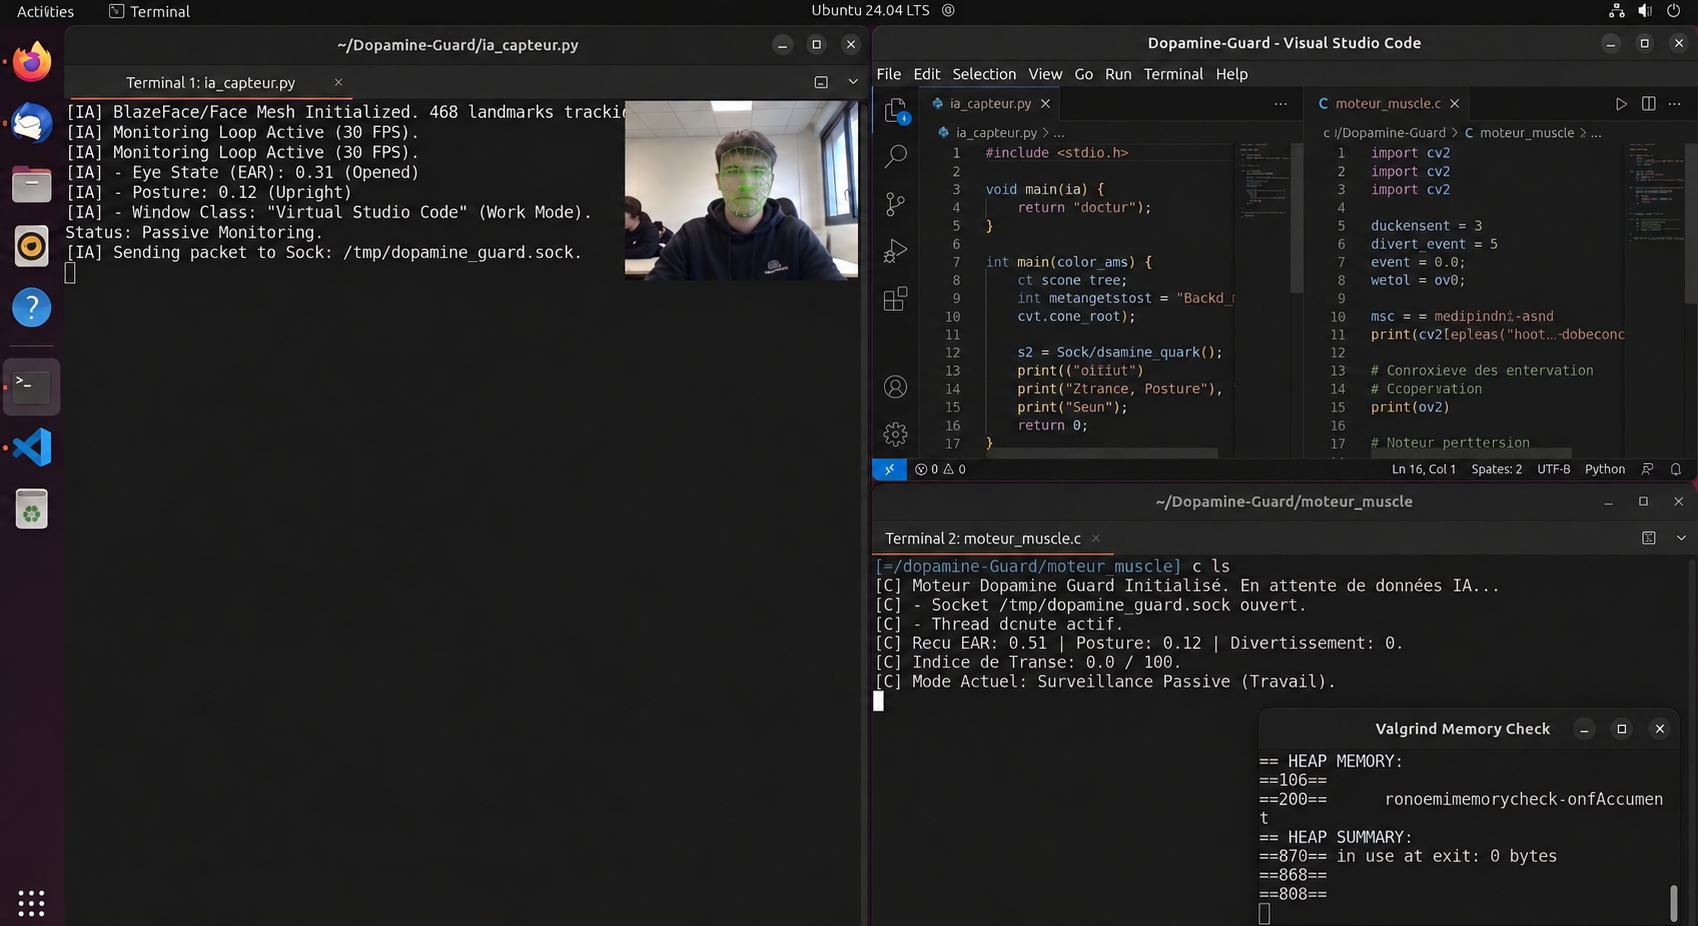
\includegraphics[width=0.6\textwidth]{screenshot_final.png} % Votre capture d'écran finale
\caption{Capture d'écran du programme Dopamine-Guard en cours d'exécution.}
\end{figure}

\end{document}